

%%%%%%%%%%%%%%%%%%%%%%%%%%%%%%%%%%%%%%
% Chapter title 
\chapter{Number and Expression}

% Chapter summary 
\begin{summary}
In this chapter, we will:
\begin{itemize}
    \item Write numbers using decimals, negatives, and fractions
    \item Add, subtract, multiply, and divide
    \item Expand and rewrite terms using exponents
    \item Find and approximate square and cube roots
    \item Simplify expressions in order of operations 
    \item Use variables to represent unknown quantities
    \item Evaluate variable expressions
    
\end{itemize}
\end{summary}

% Chapter contents 


%%%%%%%%%%%%%%%%%%%%%%%%%
\newpage 
\section{Numbers}

\subsection{Factors}
The \emph{factors} of any number \(n\) are the numbers that can be multiplied to get \(n\).  For example, the factors of \(8\) are \(1, 2, 4, \text{ and } 8\). When we say ``factors'', we are usually referring to positive whole-number factors. 

\begin{figure}[h!]
    \centering
    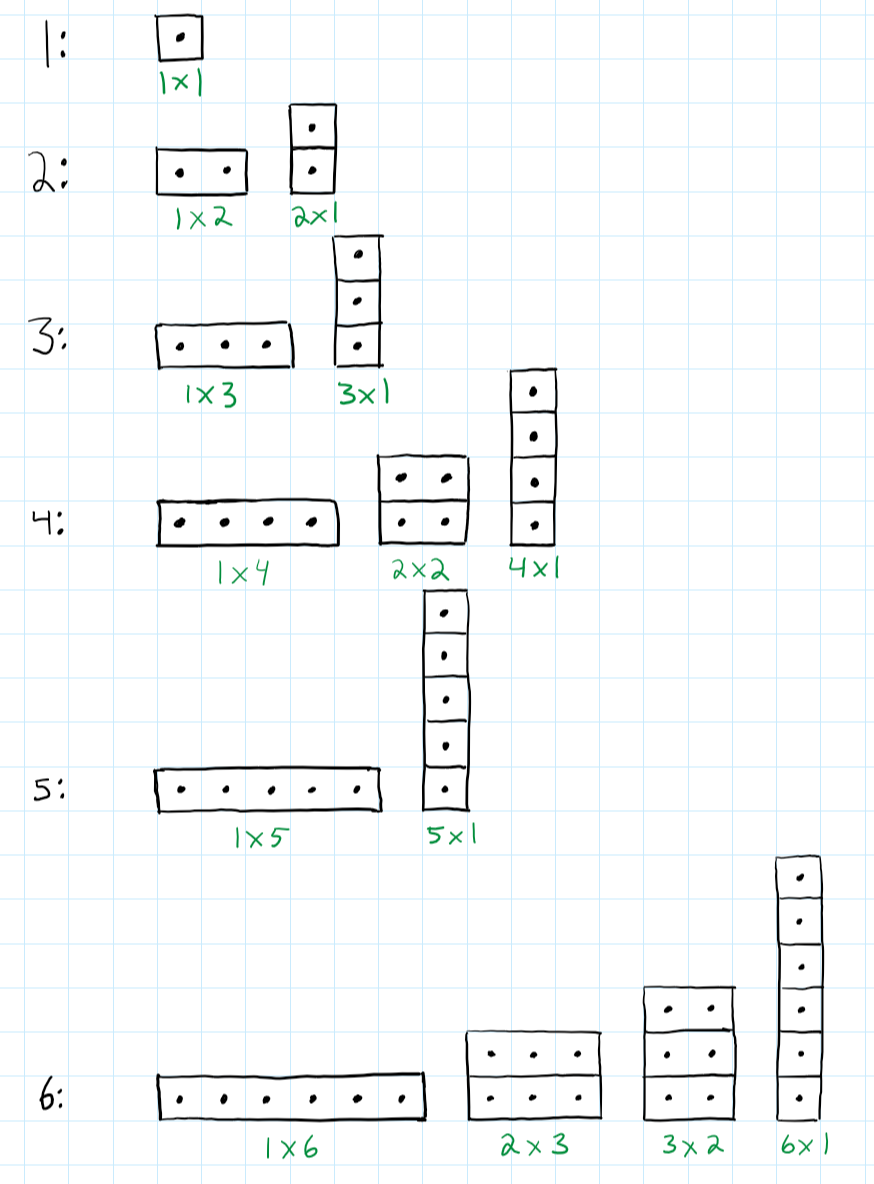
\includegraphics[width=0.7\textwidth]{img/number_factors.png}  
    % Source: Jed
    \caption{Factors diagrams for \(1\) through \(6\).}
    \label{fig:number-factors}
\end{figure}
\begin{exercise}
	Figure~\ref{fig:number-factors} depicts factoring diagrams of numbers \(1\) through \(6\).  
	Make the factoring diagrams for numbers up through at least \(18\).  
	\\ \hspace*{15mm}(a) What do you notice?
	\\ \hspace*{15mm}(b) What do you wonder? 
\end{exercise}



%%%%%%%%%%%%%%%%%%%%%%%%%
\newpage 
Observing our factoring diagrams in Figure~\ref{fig:number-factors}, some numbers can only be diagramed in two ways.  For example, \(7\) can only be written as \(1 \times 7\) and \(7 \times 1\).  In other words, the only factors of \(7\) are \(1\) and \(7\) itself.  We call such numbers \emph{prime numbers}.  Numbers that have additional number factors are called \emph{composite numbers}.   

\begin{exercise}
	Write down as many primes as you can in 1 minute!
\end{exercise}

We (humanity) know a lot about primes.  What are some questions you have about primes?

As much as we know, there is much more that we do not know!  There are many \emph{open problems} regarding prime numbers.  For example, there is no known pattern or efficient method for predicting how many numbers will pass before the next prime.  If you were to find such a pattern, you would be instantly famous!  

\subsubsection{Looking for Patterns in the Primes}
Create a list of factors for the numbers up to \(20\), and count the number of factors.  
\[ 
	\begin{array}{c | l | c}
		n & \text{Factors} & \text{Count} \\ \hline 		 
		1 & 1  & 1\\ 
		2 & 1, 2 & 2\\ 
		3 & 1, 3 & 2\\ 
		4 & 1, 2, 4 & 3\\
		5 & 1, 5 & 2 \\
		6 & 1, 2, 3, 6 & 4 \\ 
		\vdots & \vdots & \vdots  \\
	\end{array}
\]
Create a bar chart depicting the number of factors for each number starting with \(1\).  

%%%%%%%%%%%%%%%%%%%%%%%%%
\newpage 
\subsection{GCF and LCM}



%%%%%%%%%%%%%%%%%%%%%%%%%
\newpage 
\subsection{Negatives}
The negative of a number is its \emph{opposite}, and has the same distance from zero on the number line.  The opposite of \(58\) is \(-58\).  The opposite of \(-27.3\) is \(27.3\).  
% Plot the following numbers on the number line...

While not the same as subtraction, negative numbers can be viewed as positive numbers being subtracted from \(0\), an idea that will be useful when we start to perform arithmetic with negative numbers.  

\subsubsection{Adding and Subtracting} 
Adding a positive number is equivalent to moving ``right'' or ``up'' the number line.  
Draw a number line diagram for each of the operations below. 
\[10 + 2 = 12  \]
%\[80+19 = 99   \]
\[ 108 + 15 = 123  \]
%\[  -8 + 3 = -5 \]
\[  -15 + 5 = -10   \]
%\[  -8 + 20 = 12 \]
Note that even when starting with a negative, adding a positive number still moves ``up''. 

Subtracting a positive number is equivalent to moving ``left'' or ``down'' the number line. 
Draw a number line diagram for each of the operations below. 
\[ 38 - 11 = 27 \]
\[  5-8 = -3  \]
\[  -7 - 4 = -11   \]
Adding a negative can be translated to subtraction.  For example, 
\[10 + (-2) = 10 -2 = 8 \]
\[  17 + (-8) = 9 \]
Subtracting a negative can be translated to addition.  For example, 
\[  22 - (-4) = 26 \]
\[ -7 - (-2) = -5 \]

\subsubsection{Multiplying and Dividing} 
There are four cases to consider: 
\[ (+)(+) \to (+)  \]
\[ (+)(-) \to (-)  \]
\[ (-)(+) \to (-)  \]
\[ (-)(-) \to (+)  \]
Justify each of these cases for multiplication.  The same justifications will hold for division.  

%%%%%%%%%%%%%%%%%%%%%%%%%
\newpage 

\begin{exercise}
	Draw a number line diagram for each of the following operations:   \\ \\
(a)	\[  12 + 7  \]    
(b)	\[  8 + (-10) \]  
(c)	\[  -3 - 4  \]
(d)	\[  -2 - (-7)    \]

\end{exercise}


%%%%%%%%%%%%%%%%%%%%%%%%%
\newpage 
\subsection{Fractions}
There are many ways to think about fractions: we can talk about fractions as part of a whole, or as a ratio, or rate, or as division.  
\begin{figure}[h!]
    \centering
    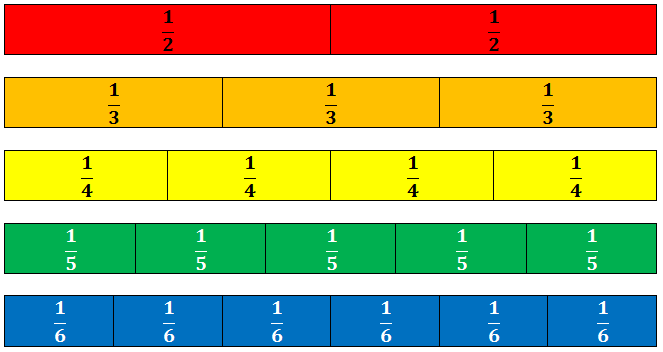
\includegraphics[width=0.7\textwidth]{img/FractionStrips.png}  
    % Source: https://commons.wikimedia.org/wiki/File:FractionStrips.PNG 
    \caption{Fraction Strips. The width is a whole.}
    \label{fig:fraction-strips}
\end{figure}
\\
A lot of concepts we'll work with revolve around \emph{equivalent fractions}, fractions that are equivalent!
\begin{figure}[h!]
    \centering
    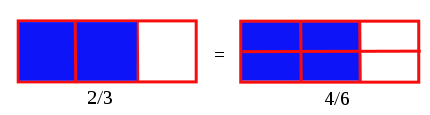
\includegraphics[width=0.5\textwidth]{img/fraction2-3.png}
    % Source: https://commons.wikimedia.org/wiki/File:Fraction2_3.svg
    \caption{Equivalent Fractions.  The fraction \(\frac{2}{3}\) is equivalent to the fraction \(\frac{4}{6}\).}
    \label{fig:equivalent-fractions}
\end{figure}
\\ 
% REDUCE 
\textbf{Reducing Fractions}
\\ \\ 
\emph{Reducing} is one of the most common tasks we'll see with fractions.  Reducing a fraction means to write a fraction in its lowest terms.  




%%%%%%%%%%%%%%%%%%%%%%%%%%%%%%%
\newpage 
\textbf{Adding and Subtracting Fractions}
\\ \\
Adding fractions involves combining numerators.   The example below could be read as ``five eigths plus two eigths equals seven eigths''.  
\begin{example}
	Find the following sum:
	\[\frac{5}{8}+\frac{2}{8}\]
\textbf{Solution:}
	\[\frac{5}{8}+\frac{2}{8} = \frac{5+2}{8} =  \frac{7}{8}\]
\end{example}
Subtraction is similar. 
\begin{example}
	Find the following difference:
	\[\frac{5}{8}-\frac{2}{8}\]
\textbf{Solution:}
	\[\frac{5}{8}-\frac{2}{8} = \frac{5-2}{8} = \frac{3}{8}\]
\end{example}
Adding and subtracting fractions requires a common denominator.  For example, we cannot cannot directly add or subtract thirds with fifths.  However, we can convert fractions to equivalent fractions with common denominators.  
\begin{example}
	Find the following sum: 
	\[\frac{7}{3} + \frac{2}{5}\]
\textbf{Solution:}
	\[\frac{7}{3} + \frac{2}{5} = \frac{35}{15} + \frac{14}{15} = \frac{49}{15} \]
\end{example}
To get a common denominator, you want to determine the smallest common multiple of your two denominators.  That is, the smallest number that is a multiple of both denominators.  In the example above, \(15\) is a multiple of both \(3\) and \(5\).  
\begin{remark}
 	When converting a fraction to an equivalent fraction, we can think of this manipulation as multiplying by \(1\).  For example, we coverted \(\frac{7}{3}\) to \(\frac{35}{15}\) by multiplying \(\frac{7}{3}\) by \(\frac{5}{5}\).  Importantly, \(\frac{5}{5} = 1\)  and multiplying by \(1\) does not change the \emph{value} of the original number. 
\end{remark}



%%%%%%%%%%%%%%%%%%%%%%%%%%%%%%%
\newpage 


\begin{exercise}
	Find the missing terms of these sums. 

	(a)	\[\frac{5}{12} + \frac{1}{12} = \frac{ }{12} \]
	(b)	\[\frac{ }{9} + \frac{2}{9} = \frac{13}{9} \]
	(c)	\[\frac{4}{3} + \frac{11}{3} = \text{---} \]
%	{\footnotesize \url{https://www.khanacademy.org/math/cc-fourth-grade-math/imp-fractions-2/imp-adding-and-subtracting-fractions-with-like-denominators/e/adding_fractions_with_common_denominators}}
\\ 
	{\footnotesize \url{https://www.ixl.com/math/grade-4/add-fractions-with-like-denominators-using-area-models}}
\end{exercise} 
\begin{exercise}
	Find the missing terms in these differences.  
	
	(a)	\[\frac{5}{12} - \frac{1}{12} = \frac{}{12} \]
	(b)	\[\frac{7}{9} - \frac{2}{9} = \text{---}  \]
	(c)	\[\frac{11}{3} - \frac{-4}{3} = \text{---} \]
\\ 
%	{\footnotesize \url{https://www.khanacademy.org/math/cc-fourth-grade-math/imp-fractions-2/imp-adding-and-subtracting-fractions-with-like-denominators/e/subtracting_fractions_with_common_denominators}}
	{\footnotesize \url{https://www.ixl.com/math/grade-4/subtract-fractions-with-unlike-denominators}}
\end{exercise} 
\begin{exercise}
	Find the missing terms in these sums and differences.  
	
	(a)	\[\frac{5}{6} + \frac{1}{2} = \frac{5}{6} + \frac{}{6} = \frac{}{6} \]
	(b)	\[\frac{7}{9} - \frac{2}{9} = \text{---}  \]
	(c)	\[\frac{11}{3} - \frac{4}{3} = \text{---} \]
\\ 	
	{\footnotesize \url{https://www.ixl.com/math/grade-6/add-and-subtract-fractions-with-unlike-denominators}}
\end{exercise} 
Additional Practice: 
\begin{itemize}
	\item {\footnotesize \url{https://www.ixl.com/math/grade-3/add-and-subtract-fractions-with-like-denominators}}
	\item {\footnotesize \url{https://www.ixl.com/math/grade-4/add-3-or-more-fractions-with-unlike-denominators}}
\end{itemize}





%%%%%%%%%%%%%%%%%%%%%%%%%%%%%%%
\newpage 
\textbf{Multiplying and Dividing Fractions}
\\ \\ 
Unlike addition and subtraction, multiplication and division of fractions does not require common denominators.  





%%%%%%%%%%%%%%%%%%%%%%%%%
\newpage 
\section{Operations}

Adding, subtracting, multiplying, and dividing are all \emph{operations} on numbers.  In this section, we'll see some additional operations including exponentiation, square roots, and cube roots.  

%\subsection{Multiplying and Dividing}
\subsection{Exponents and Roots} 
\subsection{Order of Operations}
\subsection{Application: Pythagorean Theorem} 



%%%%%%%%%%%%%%%%%%%%%%%%%
\newpage 
\section{Expressions}

\subsection{Variables}
\subsection{Evaluating Expressions}
\subsection{Equivalent Expressions}
\subsubsection{Combining Like-Terms}

%%%%%%%%%%%%%%%%%%%%%%%%%
\newpage 
\section{Exercises} 

Online Practice from this Chapter ... 

Additional problems. 















